\section{結果}
% --- experiment.tex から移動 ここから
\subsection{一層目の重みの学習}
\begin{figure}[hbt]
\centering
\begin{minipage}{0.45\columnwidth}
  \centering
  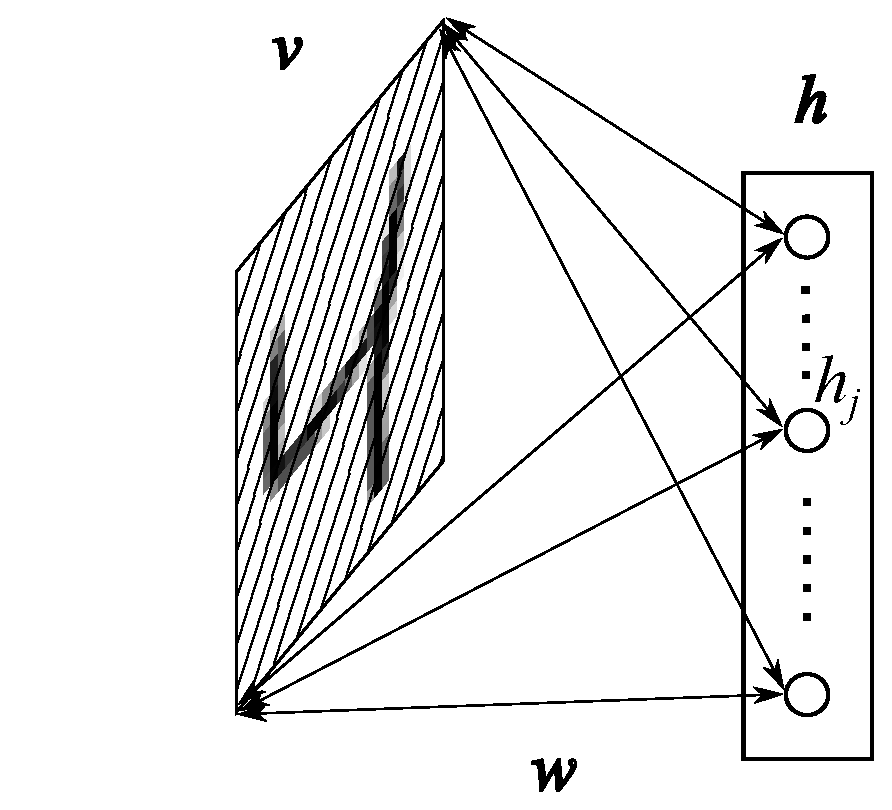
\includegraphics[width=0.8\columnwidth]{lookall_network_v7.eps}
  \caption{実験1のRBM}
  \label{cap:lookall_network}
\end{minipage}
\begin{minipage}{0.45\columnwidth}
  \centering
  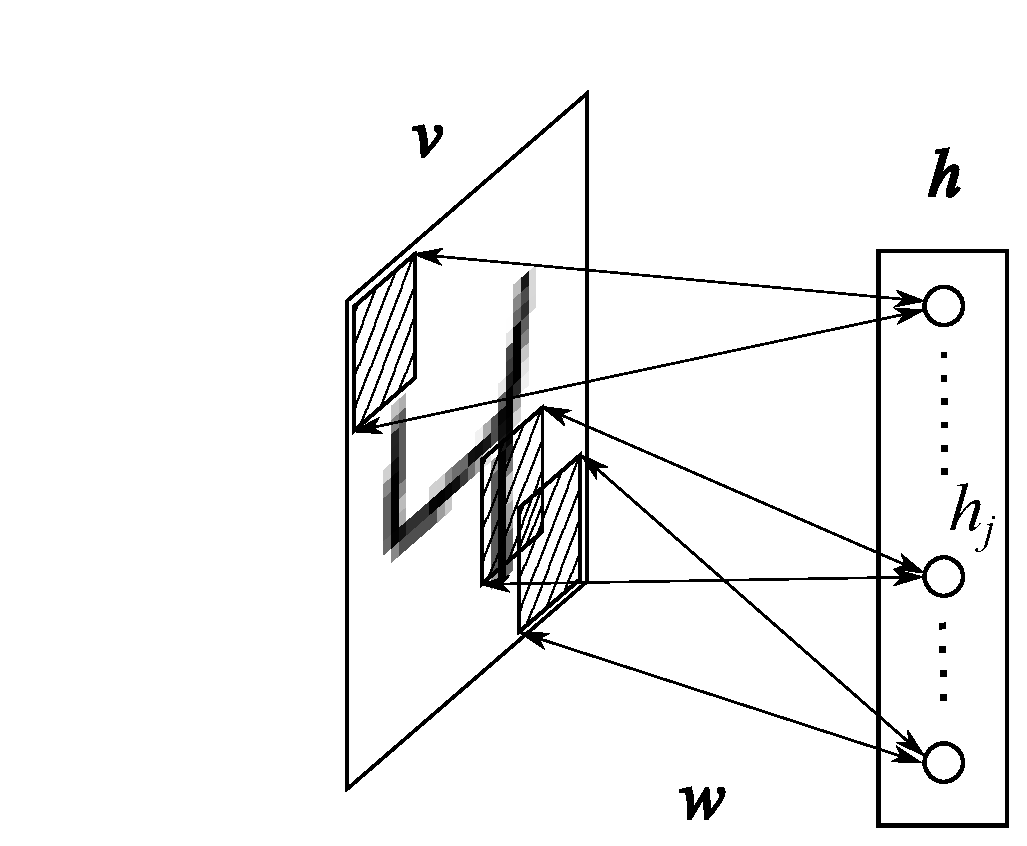
\includegraphics[width=0.9\columnwidth]{lookpartial_network_v8.eps}
  \caption{実験2のRBM}
  \label{cap:lookpartial_network}
\end{minipage}
\end{figure}
\subsubsection{実験1}
%\subsubsection{隠れ層1の素子と可視層の素子が全て結合しているRBM}
図~\ref{cap:lookall_network}のような,
可視層が$784$次元,隠れ層が$500$次元のRBMにて
手書き文字2000枚を用いて
学習率$0.001$で$1000$回の学習をした.
隠れ層の素子${h_j}$は,図~\ref{cap:lookall_network}の斜線で示した
可視層の素子$v_i$すべてと結合している.
\begin{table}%[htb]
\begin{center}
  \caption{各実験における正答率}
  \label{tab:result}
  \begin{tabular}{cccc}
    \hline
    実験   & Training set & Test set\\
    \hline \hline
    実験1  & 89.08\%      & 88.69\% \\
    実験2  & 87.34\%      & 88.36\% \\
    実験3  & 91.86\%      & 91.55\% \\
    \hline
  \end{tabular}
\end{center}
\end{table}

